\chapter{Statistics - Bayesian}

Spectroscopy is a great starting point for Bayesian statistics to those who're interested in astronomy. This is because it has plenty of data points along the $ x $-axis (e.g., wavelength) with error-bars, and we usually fit a simple analytic function to the dataset. 

Consider you have the 1-D spectrum as in \cref{fig:greco2018f2-rep}. The big question is this: \textbf{How likely is that the peak is an actual line(s), not due to random noise?}
\begin{figure}[ht!]
  \centering
  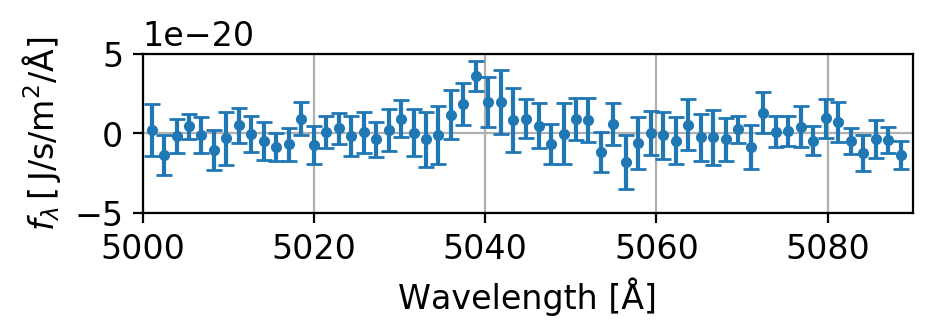
\includegraphics[width=0.6\linewidth]{figs/Greco2018F2-rep}
  \caption{The data extracted from \href{https://ui.adsabs.harvard.edu/abs/2018ApJ...866..112G/abstract}{Greco+2018ApJ}, without Gaussian fit. Note that $ 1 \,\mathrm{erg/s/cm^2/\AA} = 1 \, \mathrm{mW/m^2/\AA} $. See the notebook \texttt{Spectroscopy\_Simulation} for the codes I used in this chapter.}
  \label{fig:greco2018f2-rep}
\end{figure}


To test this, let's set up hypotheses: The null hypothesis ($H_0$) is that there is no line, while the alternative hypothesis ($H_1$) is that there \textit{is} a line\footnote{Reminder: \textit{the null hypothesis is what we want to reject}.}. Note that we haven't specified the properties of the line (amplitude, width, etc) yet. Then our strategy must be
\begin{enumerate}
\item We have to check which hypothesis is more likely (assuming there're only two possibilities, $ H_0 $ and $ H_1 $).
\item If $H_0$ is more likely, we accept the null hypothesis, i.e., ``we argue the non-existence of line in this data with certainty of xxx''.
\item If $H_1$ is more likely, we have to find the line properties (amplitude, width, etc) in the form of $ x \pm dx $.
\end{enumerate}
The first is called the \textbf{Model Selection} and the third is called the \textbf{Parameter Estimation}. If the second is the case, things are simple: no line! That's all. Model selection is \textit{discrete} (finite number of different hypotheses), while parameter estimation is usually \textit{continuous}.

\section{Bayes Theorem}
\begin{thm}[Bayes' Theorem]
If $H$, $D$, and $I$ are the hypothesis, data, and prior information, respectively, Bayes' theorem states 
\begin{equation}\label{eq: bayes thm}
  P(H | D, I) = \frac{P(H|I) \times P(D|H, I)}{P(D|I)} ~.
\end{equation}
Usually it is simply put as 
\begin{equation}\label{eq: bayes thm propto}
  P(H | D, I) \propto P(H|I) \times P(D|H, I) ~.
\end{equation}
\end{thm}
The \textbf{posterior} $P(H|D, I)$ is understood as ``the probability that the hypothesis is true, given the data equals to $D$ and we have prior information $I$.'' The \textbf{prior} $P(H|I)$ can be quite subjective, since it means ``the probability that the hypothesis is true.'' In most cases, we take either uniform prior or Jeffrey's prior (see below). The denominator, $P(D | I)  := \int P(D | H, I) P(H|I) dH$ is understood as the normalization constant for the posterior. 

The term $P(D|H, I)$ is called the \textbf{likelihood}, and this is what we have calculated during our high school course works: 

\begin{ex}[High school exam problem: calculating liklihood]
Given the hypothesis that a person has possibility 0.5 to win a game, what is the probability for her to win 3 games in a row?

In this case, the hypothesis is $H = (p=0.5)$, and the data $D = (\mathrm{win~3~in~a~row})$. The prior knowledge is that ``the game rule does not change'', ``the person doesn't use faul measures to make the possibility to change over time'', etc, which are just trivial assumptions. Most importantly, we have to assume that the results of each game should be \textit{independent}, so that we can use the multiplication law. Therefore,
\begin{equation*}
  P(D|H, I) = (1/2)^3 = 1/8 ~.
\end{equation*}

In real scientific problems, $I$ can be something like ``the fundamental physical laws do not change over time'', ``this galaxy is spiral for sure (if you're working on rotational curves of S galaxies, you may assume your samples are definitely S, not E or Irr)'', etc.
\end{ex}

When you are finding the mean of the data, it is a single parameter case, and therefore, $ H $ just means the mean value, so you can write something like this: $ P(H|D, I) = P(m|D, I) $. When you have multiple parameters, usually people denote the set of paramers as $ \vec{\theta} $, so $ P(H|D, I) = P(\vec{\theta}|D, I) $. If we're fitting the data with, say, a 3rd order polynomial with 4 parameters, we can understand that $ I $ includes ``the data is described by a 3rd order polynomial with 4 parameters''. 

\section{Towards the Model Selection}
\subsection{Model Selection Concept}
The term ``odd'' is used for $ \frac{\mathrm{probability}}{1 - \mathrm{probability}} $. In this case the $ P(H_1|I) / P(H_0|I) $ is called the prior odds because $ P(H_1|I) + P(H_0|I) = 1$, as there is no other possibility other than $ H_0 $ and $ H_1 $. Similarly, since $ P(D|H_0, I) + P(D|H_1, I) = 1$, the LHS is also called the posterior odds.

Now come back to the original question: model selection. The model selection is done based on the \textbf{odds ratio}:
\begin{equation}\label{eq: odds ratio}
  R := \frac{P(H_1 | D, I)}{P(H_0 | D, I)}
    = \frac{P(H_1|I)}{P(H_0|I)} \times \frac{P(D|H_1, I)}{P(D|H_0, I)} 
    = \mathrm{odds}(\mathrm{prior}) \times B_{10}~.
\end{equation}
Here $ B_{10} $ is called the \textbf{Bayes' factor}. 

If $ R > 1 $, we select $H_1$ over $H_0$ and vice versa. If $R=1$, we can't give any conclusion. Equivalently, we can use $\ln R $ and compare it with 0. This is because we frequently get extremely large or small $R$ values (e.g., $10^{-40}$), which is inappropriate for some computer programming.


\subsection{Prior Selection}
There are two major priors: uniform and Jeffreys' prior.
\begin{itemize}
\item \textbf{Uniform prior} assumes uniform probability for the model within reasonable range. 
\item \textbf{Jeffreys' prior} assumes the probability proportional to the determinant of the Fisher information matrix. Simply put, for the parameters like standard deviation, if the value is small (has more information), we give more weight to it.
\end{itemize}
Another possibility is that iteratively updated prior based on the accumulated data, as sometimes used in artificial intelligence.

\begin{ex} [Uniform prior]
Consider an emission line fitting to the 1-D spectrum. If you are sure that the line must be Gaussian with center $ \lambda_c \in [650, 655]\,\mathrm{nm} $, the uniform prior of the line center will be $ \lambda_c \sim \mathcal{U}(650, 655) $, which has the pdf of $ p(\lambda_c) = 1/5 $ for $ \lambda_c \in [650, 655]\,\mathrm{nm} $ and 0 otherwise. That is, uniform prior regards it is equally likely to have any value within the bound specified by the user.
\end{ex}

%\begin{ex} [Jeffereys' prior]
%Jeffereys' prior is suitable for parameters like scatter of the data. For instance, for a set of $ N $ samples which show a Gaussian distribution of the single-valued population. An example is like this: You make multiple measurements of the standard star's magnitude, which must be a constant over the time, to understand how accurately your instrument can measure the stellar magnitude, i.e., the stability of the instrument.
%\end{ex}
%That is, if the parameter is small, we give more weight to it; this is similar to the information theory which gives higher weight if a data is "unlikely". For this reason, we usually use Jeffrey's prior for standard deviation estimation. Quantitatively, it is $ P(A|I) = \frac{1}{A \log_e(75/25)}$. This is understood as the uniform prior of the log of $A$: $P(\log_e A| I) d(\log_e A) = \frac{d(\log_e A)}{\log_e A_{max} - \log_e A_{min}} $ $\rightarrow P(\log_e A| I) = \frac{1}{A \log_e (A_{max}/A_{min})}$ .

%Since Jeffrey's prior is non-sensical when we include model of $A=0$, a **modified Jeffrey's prior** is also used: $ P(A|I) = \frac{1}{A+A_0} \times \frac{1}{\log_e \frac{A_0+A_{max}}{A_0+A_{min}}} $. This is nothing but a parallel shift of parameters by a certain constant $A_0$. $A_0$ can be taken as a noise level, such as readout noise in our case.


\subsection{Likelihood Calculation}
Assume all data values, e.g., the $ f_\lambda $ values, are independent\footnote{A strange thing happens on CCD sometimes maybe? If this is true, then nothing is independent. See \href{https://ui.adsabs.harvard.edu/abs/2018PASP..130f4504B/abstract}{BooneK+18 PASP} (\texttt{2018PASP..130f4504B}) ``A Binary Offset Effect in CCD Readout and Its Impact on Astronomical Data
''.}. Denoting the $ i $-th pixel's value as $ D_i $, %. Applying the product rule to independent measurements,
\begin{equation*}
  P(D|H, I) = P(D_1, \cdots , D_N | H, I) = P(D_1 | H, I) \times \cdots \times P(D_N | H, I) ~.
\end{equation*}

Under $H_0$ (no emission line), $P(D_i | H_0, I) $ is the probability to measure $D_i$ electrons when there is only the pixel noise $\sigma_i$ (no actual line). Each pixel we have Poissonian noise which is nearly Gaussian, and sky estimation noise term, which is difficult to quantify but we usually assume it is Gaussian, and the Gaussian readout noise in standard CCD. Therefore, each pixel is assumed to have a Gaussian noise. Thus,
\begin{equation*}
  P(D_i | H_0, I) = \frac{1}{\sqrt{2 \pi} \sigma_i} \exp{ \left ( -\frac{(D_i - 0)^2}{2 \sigma_r^2} \right )} 
  \quad\rightarrow\quad
  P(D|H_0, I) =  \prod_{i=1}^{N} P(D_i | H_0, I)
\end{equation*}
Then the \textbf{log-liklihood} is
\begin{equation}\label{eq: log-l H0}
  \ln P(D|H_0, I)
    = C_\sigma
      - \sum_{i=1}^{N} \frac{D_i^2}{2 \sigma_i^2} ~,
\end{equation}
where $ C_\sigma := \sum \ln (\sqrt{2 \pi} \sigma_i)^{-1} $ is a constant. Note that even the second term is a calculable constant once the data is given.

For $H_1$, we can just change the zero mean to the Gaussian line profile. Consider the best-fit line profile is described as $ g(x| \vec{\theta}_0) $ for $ \vec{\theta}_0 = (A, w, \lambda_c) $ (amplitude, width sigma, central wavelength). Then
\begin{equation}\label{eq: log-l H1}
  \ln P(D|H_1, I)
    = C_\sigma
      - \sum_{i=1}^{N} \frac{(D_i - g(x_i|\vec{\theta}_0))^2}{2 \sigma_i^2} 
    \equiv C_\sigma - \frac{1}{2}\chi^2
      ~.
\end{equation}
Here, $ \chi^2 $ is the usual chi-square statistic from the data and model, because in our case, the error-bars are independent and normally distributed. Finding the best-fit parameter set, $ \vec{\theta}_0 $, is done by the least-square fitting (also called the $ \chi^2 $-minimization). 

Although it is mathematically too trivial, let me put another theorem to emphasize.
\begin{thm}
Maximizing (log-)likelihood is identical to minimizing $ \chi^2 $, when the error-bars are independent and follows Gaussian.
\end{thm}

\subsection{Model Selection Calculation}
Now let's do the real calculation to compare $H_0$ and $H_1$. Because I want to use amplitude rather than flux as a free paramter, the gaussian function will be $ g(x|\vec{\theta}_0) = A e^{-(\lambda - \lambda_c)^2/2w^2} $. The best fit Gaussian function to the data shown in \cref{fig:greco2018f2-rep} is found to have the following parameters:
\begin{equation}
  \mathrm{amplitude} = 3.213 \times 10^{-20}
  \quad;\quad
  \lambda_c = 5039.4 \,\mathrm{\AA}
  \quad;\quad
  w = 2.33 \,\mathrm{\AA}
\end{equation}
with the integrated flux $ \lg (F_\mathrm{O_{III}} / \mathrm{mW\, m^{-2}}) = -15.73 $, because $ F = A \sqrt{2\pi w^2} $. This matches well with the original publication $ -15.7 \pm 0.1 $. 

From the data, $ C_\sigma = 2739.234 $. The log-likelihood of $ H_0 $ and $ H_1 $ are
\begin{align*}
  \ln P(D|H_0, I)
    &= C_\sigma
      - \sum_{i=1}^{N} \frac{D_i^2}{2 \sigma_i^2}
    &&= 2720.810 \\
  \ln P(D|H_1, I)
    &= C_\sigma
      - \sum_{i=1}^{N} \frac{(D_i - g(x_i|\mathrm{amplitude}, \lambda_c, w))^2}{2 \sigma_i^2} 
    &&= 2730.136 ~.
\end{align*}

Assume the probability of $ H_0 $ being true is the same as that of $ H_1 $ being true. The  Bayes' ratio in \cref{eq: odds ratio} therefore becomes just a Bayes' factor:
\begin{equation}
  R = B_{10} = \frac{e^{2730.136}}{e^{2720.810}} = 1.12 \times 10^{4} \gg 1 ~,
\end{equation}
which means $ H_1 $ is extremely more likely. Thus, we now believe there must be an emission line, and have to find the CI of the parameters (e.g., flux value). 


\subsection{Model Selection with AIC, BIC}
But wait, is this all? No.

The pitfall of this na\"{i}ve approach using Bayes' ratio is that, you can minimize $ \chi^2 $ to 0, by increasing the number of fitting parameters. When the number of free parameters is equal to the number of data points, you must be able to make a function $ f $ such that $ D_i - f(\lambda_i) $ is always 0. Does the $ N $-parameter model a better choice than 1-parameter case, for example, if just the ratio is large? It can't be.

The ``number of paramter'' problem is not an easy thing to solve, but we have simple rule-of-thumbs: The Akaike Information Criteria, AIC, and the Bayesian Information Criteria, BIC. The derivations are not shown here, because it can become a bit lengthy while that derivation itself is not at the heart of the understanding.

\begin{thm}[Bayesian Information Criterion; BIC]
For the $ N (\rightarrow \infty) $ data points, the BIC for the model with $ n $ free parameters denoted as $ \vec{\theta} $ is given as
\begin{equation}\label{eq: bic}
  \mathrm{BIC} := n \ln N - 2 \ln P(D|\vec{\theta}_0, I) = n \ln N + \chi^2_\mathrm{min} - 2C_\sigma ~,
\end{equation}
where $ \vec{\theta}_0 $ is the best-fit parameter which results in the minimum $ \chi^2 $, or maximum likelihood ($ P(D|H, I) $).
For the same data, comparing with two different models, the difference in the BICs is used:
\begin{equation}\label{eq: dbic}
  \Delta \mathrm{BIC} 
    = (n_1 - n_2) \ln N 
      - 2 \ln \frac{P(D|\vec{\theta}_{0, 1}, I)}{P(D|\vec{\theta}_{0, 2}, I)}
    = (n_1 - n_2) \ln N 
      + (\chi^2_\mathrm{min, 1} - \chi^2_\mathrm{min, 2}) ~.
\end{equation}
The second equalities above including $ \chi^2 $ hold only if the error-bars are independent and normally distributed.

Some people prefer to define in the opposite sign and/or half of this value to remove the factor 2 in front of the log-likelihood.
\end{thm}
Note that BIC is usable only if $ N \gg n $. Also the prior distribution only affects when you find $ \vec{\theta} $, not when calculating the BIC. 

Since RafteryAE's work\footnote{RafteryAE (1995) ``Bayesian Model Selection in Social Research'', Sociological Methodology, 25, 111}, the following criteria for choosing models are widely used:

\begin{table}[ht!]
\centering
\label{tab: bic}
\begin{tabular}{|c|c|c|c|c|}
  \hline 
  $ |\Delta\mathrm{BIC}| \in $ & [0, 2] & [2, 6] & [6, 10] & 10+ \\ 
  \hline 
  Evidence & Not worth more than a bare mention & Positive & Strong & Very Strong \\ 
  \hline 
\end{tabular}  
\end{table}


\begin{thm}[Akaike Information Criterion; AIC]
For the $ N (\rightarrow \infty) $ data points, the BIC for the model with $ n $ free parameters denoted as $ \vec{\theta} $ is given as
\begin{equation}\label{eq: aic}
  \mathrm{AIC} := 2n - 2 \ln P(D|\vec{\theta}_0, I) = 2n + \chi^2_\mathrm{min} - 2C_\sigma ~,
\end{equation}
where $ \vec{\theta}_0 $ is the best-fit parameter which results in the minimum $ \chi^2 $, or maximum likelihood ($ P(D|H, I) $). 
For the same data, comparing with two different models, the difference in AICs is used:
\begin{equation}\label{eq: daic}
  \Delta \mathrm{AIC} 
  = 2(n_1 - n_2) - 2 \ln \frac{P(D|\vec{\theta}_{0, 1}, I)}{P(D|\vec{\theta}_{0, 2}, I)}
  = 2(n_1 - n_2) + (\chi^2_\mathrm{min, 1} - \chi^2_\mathrm{min, 2}) ~.
\end{equation}
The second equalities above including $ \chi^2 $ hold only if the error-bars are independent and normally distributed.
\end{thm}

Although I am not so familiar with hard-core statistics, it seems like there are debates about which should be preferred (BIC or AIC). BIC is known to prefer the ``true model'', if it is in our set of alternative hypotheses, with probability 1 when $ N \rightarrow \infty $, while AIC doesn't. On the other hand, if the data is too few (note that the difference in BIC and AIC is the $ \ln N $ term), BIC tend to seek for the model which explains that small dataset, so it can prefer worse model which tries to explain the bad data points than AIC. 

Now let's calculate $ \Delta \mathrm{BIC} $ and $ \Delta \mathrm{AIC} $ for our sample data to test $ H_0 $ VS $ H_1 $. As before, $ C_\sigma = 2739.234 $, and log-likelihoods are 2720.810 and 2730.136. Then because $ H_0 $ has no parameter and $ H_1 $ has three paramters, and $ N = 61 $,
\begin{align*}
  \Delta \mathrm{BIC}
    &= (0 - 3) \ln 61 - 2 (2720.810 - 2730.136)
    &&= 6.32 \\
  \Delta \mathrm{AIC}
    &= 2 (0 - 3) - 2 (2720.810 - 2730.136)
    &&= 12.65
\end{align*}
The fact that these are positive means we should prefer the $ H_1 $, but not as strong as what we've seen from the odd's ratio.


\section{Towards the Parameter Estimation}

\subsection{Brute-Force}
From the last section, we learned we have a clear evidence that there is a line. Then how can we estimate the line properties with uncertainties? This is the same as we did in the statistics chapter. First is the \textbf{brute-force} fixed-grid search scheme

In the chi-square sense, what we have to do are
\begin{enumerate}
\item Calculate the chi-square statistic at each parameter space position. 
\item Keep only those with $\chi^2 < \chi^2_\mathrm{min} + \Delta(n_\theta, \alpha)$ 
  \begin{enumerate}
  \item [-] $\Delta$: inverse cdf (cumulative distribution function) of $\chi^2$ distribution.
  \item [-] $\alpha$: significance level ($\alpha = 0.6827$ for 1-sigma)
  \item [-] $ n_\theta $: number of free parameters.
  \item [-] In python, you can do \pyth{delta = scipy.stats.chi2.ppf(0.6827, n_param)}
  \end{enumerate}
\item These are the models ``within 1-sigma level confidence interval.''
\item Get the min/max of each of the parameters and set these as lower/upper limit of the parameters.
\item The \textit{center} of the parameters can be obtained by simple maximum likelihood estimation, such as least-square fitting.
\end{enumerate}

For the 1-sigma contour of 2 parameters, $ \chi^2 < \chi^2_\mathrm{min} + 2.30 $. The marginalized pdfs is usually drawn together to grasp the distribution of the parameters. If you have used chi-square statistic, you can use the fact that $ P \propto e^{-\chi^2/2} $. Define $ \bar{P} =  e^{-\chi^2/2}$. Then the normalization constant will be $ A = \sum_{parameters} \bar{P} $, i.e., you can use $ P = \bar{P}/A $ as the normalized probability values.

In this example, because the authors mentioned that the $ w $ parameter is obtained from the $ \mathrm{H\alpha} $ fitting, I just fixed the $ w $ value as the best fit value. From zooming in the oringinal paper, I couldn't find any difference from theirs to ours. 

\begin{figure}[ht!]
  \centering
  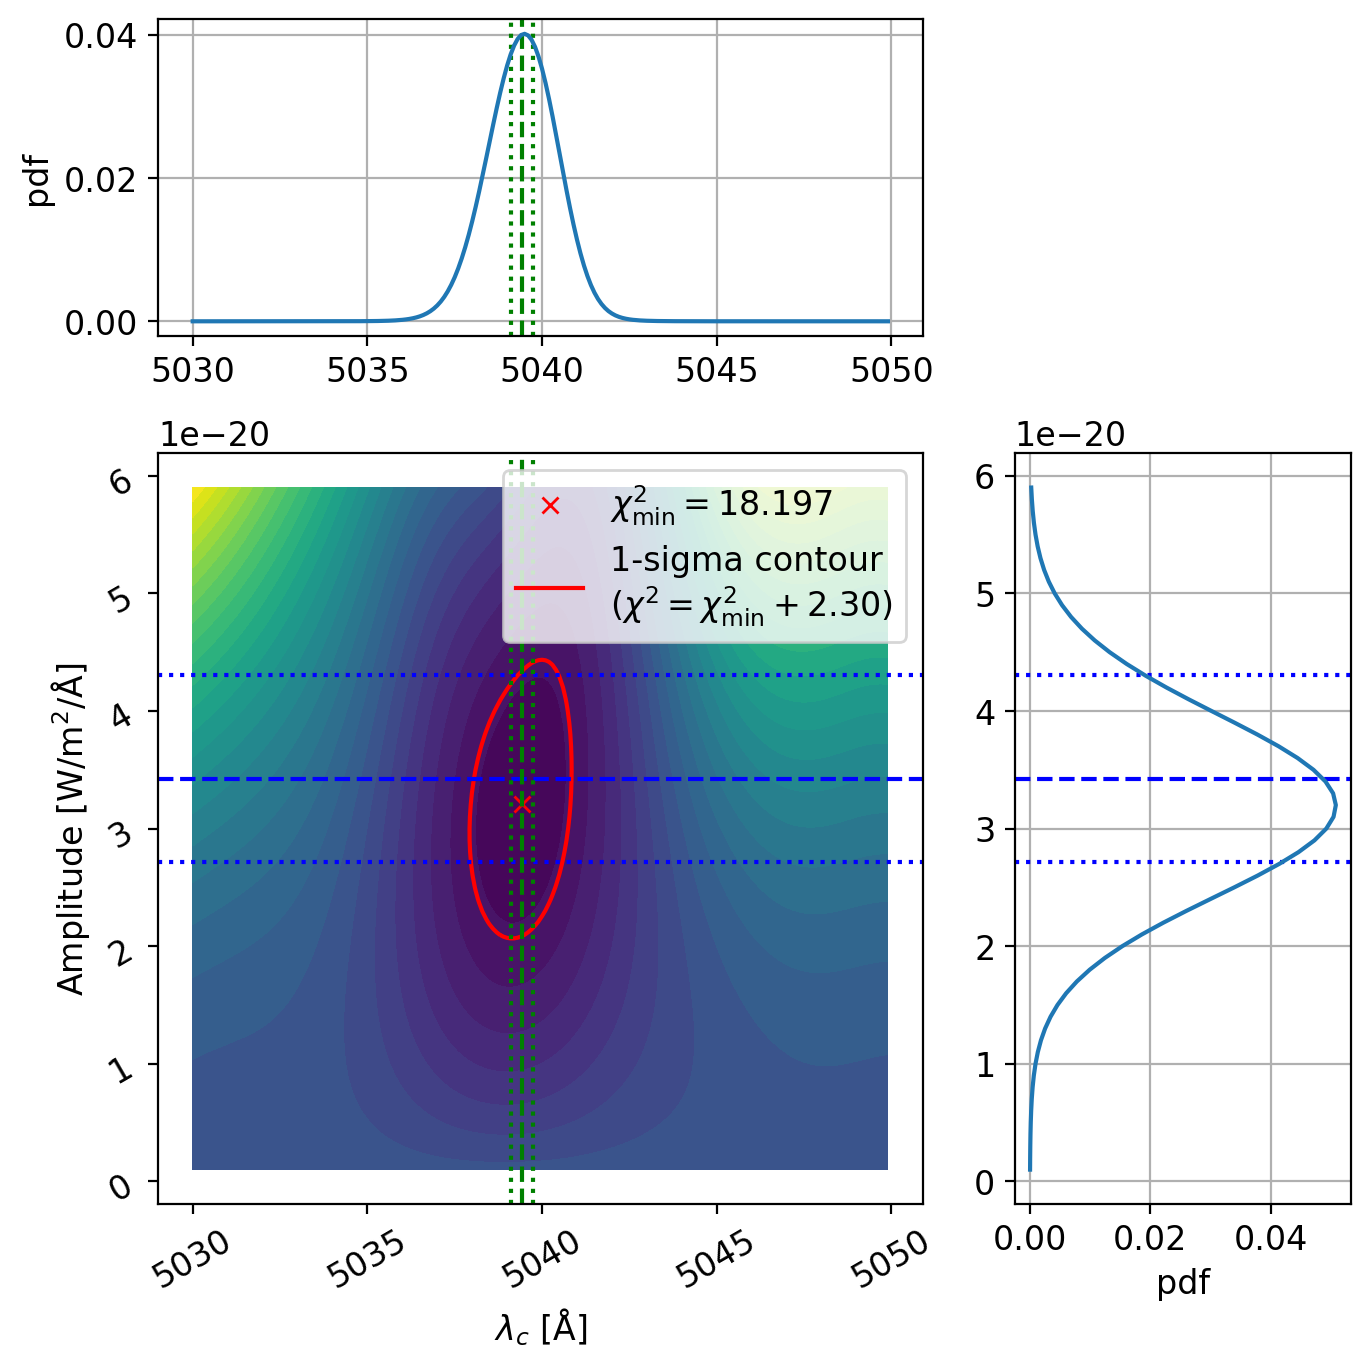
\includegraphics[width=0.7\linewidth]{figs/Greco2018-fit}
  \caption{Our fitting of Gaussian curve to the emission line. The 2-D contour shows the $ \chi^2 $ map in the 2-D parameter space. The 1-D plots show marginalized pdf from $ P = e^{-\chi^2/2} / \bar{P} $.}
  \label{fig:greco2018-fit}
\end{figure}

In the figure, the green vertical lines:
\begin{itemize}
  \item dashed = our best fit central wavelength
  \item dotted = the uncertainty range from the paper's redshift uncertainty measured from $ \mathrm{H\alpha} $ line ($ 1742 \pm 19 \,\mathrm{km/s} $)
  \item Because their uncertainty is from $ \mathrm{H\alpha} $, which has signal much better than $ \mathrm{O^{2+}} $, the error-bar is much smaller than ours.
\end{itemize}
and the blue horizontal lines:
\begin{itemize}
\item dashed = paper's flux ($ 10^{-15.7} \,\mathrm{mW/m^2} $) converted to amplitude
\item dotted = paper's uncertainty around the paper's value.
\item The difference between our fit and paper's value is only 0.03 dex (maybe the authors obtained the identical value but just dropped the significance numbers)
\item Error bars seem slightly understimated, but in reality if we use error bar of 0.14 dex in log scale, it's similar to ours. Maybe the authors just did not care about such detailed numbers, which is understandable.
\end{itemize}

\subsubsection*{Notes}
The original paper argue that they used gaussian with flat spectrum\footnote{From the paper: ``When fitting the [O III] $ \lambda $5007 line, we assume a flat continuum plus a single Gaussian line profile with standard deviation given by the $ \mathrm{H\alpha} $ fit.''}. When I tried this, however, the best fit constant is \texttt{-1.36e-21} , which must be a marginally visible negative shift to the fitted Gaussian, but I cannot find this by zooming in the paper's plot. Thus, I guess they may have just ignored this flat offset or set a bound that this constant must be positive, so that the best fit value is just 0.


\subsection{Markov Chain Monte Carlo (MCMC)}
Markov chain is a fancy name of ``memoryless'':
\begin{equation}\label{eq: markov chain}
  p(x_5|x_4, x_3, x_2, x_1) = p(x_5|x_4)
\end{equation}
The Monte Carlo (MC)\footnote{Historical background adopted from \href{https://events.mpifr-bonn.mpg.de/indico/event/30/material/slides/12.pdf}{KalinovaV's lecture note 2017 Feb}.} came from the casino ``Monte Carlo'' in Monaco. Stanislaw Ulam and John von Neumann, in 1940, wanted to find best-fit parameters to make a better nuclear weapon at the Los Alamos National Laboratory. They arrived at the idea of (now-called) Monte Carlo, but wanted it to be secret to enemies, so they chose the secret name MC, where Ulam's uncle used to play gamble. 

When you have, e.g., 7 parameters to fit 100 data points, and if the model is too complicated, the usual grid searching in the previous section is computationally impossible. Therefore, the ``hopping'' in the N-dimensional parameter space is suggested and that's MC. Currently I don't have complete plan to cover MCMC in AO class, but you may refer to many available packages from websites\footnote{A great compilation is available \href{https://gabriel-p.github.io/pythonMCMC/?fbclid=IwAR2hxgATmm1w-QFAjsjcrTbpOHeGV3aJKCCpSnnSuimEXLk9xtC3lpzXgo0}{here}}. I recommend you to try \texttt{emcee} (although I used \texttt{pymc3}, but I feel \texttt{emcee} is more standard and safe as it's classical. \texttt{pymc3} is too much a black box to my eyes, and my friends kind of agreed).


% Let me assume uniform prior to all three paramters with domains $A \in [0.1, 10]$, $\lambda_c \in [5030, 5050]$, and $w \in [0.1, 5]$, and thus $P(A|I) = (1/9.9) (^\forall A \in [0.1, 10])$, etc. Assuming all paramters are independent, we can use product rule and
%\begin{equation}
%  P(D|H_1, I) = \int_{0.1}^{5} \int_{5030}^{5050} \int_{0.1}^{10} 
%                P(D | A, \lambda_0, w, I) P(A|I) P(\lambda_0|I) P(w|I)  dA d\lambda_0 dw ~,
%\end{equation}
%
%or
%$$ \log_e P(D|H_1, I) = - \log_e (10000) + \log_e \left [ \int_{5}^{15} \int_{590}^{610} \int_{25}^{75} 
 %               P(D | A, \lambda_0, w, I) ~dA~d\lambda_0~dw \right ] ~, $$
%with 
%$$ P(D|A, \lambda_0, w, I) = \left ( \frac{1}{\sqrt{2 \pi} \sigma_r} \right )^N 
%                \times \exp \left [ -\sum_{i=1}^{N} \frac{(D_i - E_i(A, \lambda_0, w))^2}{2 \sigma_r^2} \right ] ~. $$
%Since $H_0$ has no more parameters, we just use the previous $\log_e P(D|H_0, I)$ formula.